\documentclass[conference]{IEEEtran}

\IEEEoverridecommandlockouts

% The preceding line is only needed to identify funding in the first footnote. If that is unneeded, please comment it out.

\usepackage{cite}
\usepackage{amsmath,amssymb,amsfonts}
\usepackage{algorithmic}
\usepackage{graphicx}
\graphicspath{{evals/data/metrics/figures/final/}}
\usepackage{textcomp}
\usepackage{xcolor}
\usepackage{array}
\usepackage{booktabs}
\usepackage[most]{tcolorbox}

% Churkin Protocol: Color Palette (Harmonious & Minimal)
\definecolor{churkinpurple}{RGB}{94,45,121}    % #5E2D79 (for State)
\definecolor{statusgreen}{RGB}{34,139,34}      % #228B22 (Green for True - Success)
\definecolor{statusred}{RGB}{255,99,71}       % #FF6347 (Light Red/Tomato for False - Stop/Suppressed)

\def\BibTeX{{\rm B\kern-.05em{\sc i\kern-.025em b}\kern-.08em
    T\kern-.1667em\lower.7ex\hbox{E}\kern-.125emX}}

\begin{document}

\title{EXAIM: Explainable AI Middleware for Real-Time Multi-Agent Clinical Decision Support}

\author{\IEEEauthorblockN{Abem Woldesenbet}
\IEEEauthorblockA{\textit{The Beacom College of Computer \& Cyber Sciences} \\
\textit{Dakota State University}\\
Madison, SD, USA \\
abem.woldesenbet@trojans.dsu.edu}
\and
\IEEEauthorblockN{Andy Behrens}
\IEEEauthorblockA{\textit{Information Systems, College of Business \& Information Systems} \\
\textit{Dakota State University}\\
Madison, SD, USA \\
andy.behrens@dsu.edu}
}

\maketitle

\begin{abstract}
 Clinical decision support systems (CDSS) increasingly leverage multi-agent large language model (LLM) architectures to decompose complex diagnostic reasoning into specialized components. However, these systems generate verbose, interleaved reasoning traces that are difficult for clinicians to interpret in real time, limiting transparency and clinical adoption. We present EXAIM (Explainable AI Middleware), a novel middleware architecture that transforms live multi-agent reasoning traces into structured, concise summaries aligned with clinical documentation schemas. EXAIM employs a three-layer pipeline: (1) TokenGate, a syntax-aware pre-buffer that regulates token flow using configurable word thresholds and boundary detection; (2) BufferAgent, an LLM-powered semantic boundary detector that uses structured output analysis to trigger summarization based on completeness, relevance, novelty, and topic coherence; and (3) SummarizerAgent, a schema-constrained compressor that generates summaries aligned with clinical communication frameworks (SBAR/SOAP) \cite{haig2006sbar,podder2023soap} while enforcing bounded character budgets. Unlike post-hoc explanation methods, EXAIM operates incrementally on live reasoning streams, improving information density per update in the clinician-facing update stream while preserving diagnostic transparency. Our architecture addresses critical gaps in CDSS explainability by providing process-level narrative transparency rather than feature-importance visualizations, supporting real-time clinical workflows, and maintaining multi-agent attribution. The system's modular design enables integration with existing multi-agent CDSS frameworks while remaining agnostic to specific clinical domains or agent implementations. This work contributes a reproducible, empirically evaluated approach to explainable multi-agent clinical AI, with implications for human-AI collaboration in time-sensitive medical decision-making.
\end{abstract}

\begin{IEEEkeywords}
Clinical decision support systems, explainable artificial intelligence, multi-agent systems, large language models, real-time summarization, middleware architecture, human-AI collaboration
\end{IEEEkeywords}

\section{Introduction}

Clinical decision support systems (CDSS) increasingly employ multi-agent large language model (LLM) architectures to decompose complex diagnostic reasoning into specialized components such as information retrieval, differential diagnosis, uncertainty estimation, and safety review \cite{sutton2020cdss,miyachi2023learning,chenx2025diagnostic,chen2025enhancing}. While these architectures improve diagnostic performance and robustness \cite{chenx2025diagnostic,chen2025enhancing}, they introduce a critical usability challenge: multi-agent systems generate long, interleaved reasoning traces that are difficult for clinicians to interpret during time-sensitive decision-making \cite{peng2025tree,hong2024argmed,ozgun2025psychotherapy}.



Existing approaches to explainability in clinical AI predominantly rely on post-hoc methods such as feature importance visualizations, attention maps, or static textual explanations generated after inference completion \cite{abbas2025xai,salimiparsa2021design,goel2022covid,schoonderwoerd2021patterns}. Although valuable for auditing model behavior, these methods are poorly aligned with real-time clinical workflows \cite{abbas2025xai,salimiparsa2021design,derksen2025cdss,schoonderwoerd2021patterns}. They expose internal model mechanics rather than the evolving clinical narrative \cite{benzion2025anxiety,salimiparsa2021design,hong2024argmed,schoonderwoerd2021patterns}. Furthermore, traditional explainability approaches fail to account for distributed reasoning and high-velocity, redundant trace emissions that increase output volume and cognitive overload in clinicians \cite{leduc2025speech,sanwal2025layered,hong2024argmed,wu2025incremental,hor2025design}. Recent work emphasizes that AI systems for general practice must address cognitive load through transparency that supports clinical sensemaking rather than exposing internal model mechanics \cite{hor2025design}. The update frequency in clinician-facing interfaces often results in verbose or redundant information that does not reflect the summarized treatment plan \cite{leduc2025speech,wu2025incremental,krishna2021soap}.



Conversational interfaces for multi-agent systems typically rely on turn-based interaction paradigms, surfacing outputs only at agent turn boundaries. In human-human communication, turn-taking corresponds to semantic completion; however, in multi-agent LLM systems, a single turn may contain multiple topic shifts, partial hypotheses, or exploratory reasoning. Treating turns as semantic units leads to lossy compression, redundancy, and reduced faithfulness when reasoning traces are summarized for clinical consumption. These limitations highlight the need for a real-time, process-level explainability mechanism that operates during reasoning rather than after it. Such a mechanism must regulate information flow, identify semantically meaningful update points, and present structured summaries that align with clinical communication practices while preserving attribution and uncertainty \cite{marcilly2018alerts}.

\textbf{Research Questions}


Therefore, We propose EXAIM (Explainable AI Middleware), a real-time summarization architecture designed to bridge the gap between multi-agent reasoning complexity and clinical information needs.  to improve output summarizations and reduce clinician cognitive overload. The following research questions are presented:

\textbf{RQ1:} Can event-driven, schema-constrained summarization reduce cognitive overload in LLM reasoning traces?

Following a design science research paradigm, RQ1 is investigated through the construction and evaluation of a summarization middleware artifact. The research question is operationalized via four sub-questions, each corresponding to a distinct evaluation dimension of the artifact:

\begin{itemize}
\item \textbf{RQ1a:} Does EXAIM improve global semantic trace coverage under identical schema and length constraints?
\item \textbf{RQ1b:} Does EXAIM reduce redundant and low-novelty updates while regulating update frequency?
\item \textbf{RQ1c:} Does EXAIM preserve contract-grounded faithfulness when limited continuity across summaries is permitted?
\item \textbf{RQ1d:} What impact does semantic event detection introduce relative to simpler triggers such as...?
\end{itemize}

To evaluate these questions, we conducted an ablation study in which we instantiated a real-time summarization middleware that intercepts LLM reasoning traces and emits structured summaries constrained by a fixed schema. The artifact enables controlled variation of triggering strategies (event-driven versus baseline triggers), continuity constraints, and update policies, allowing systematic assessment of their effects on semantic coverage, redundancy, faithfulness, and computational overhead.


The study builds on recent advances in incremental summarization \cite{leduc2025speech,wu2025incremental}. EXAIM operates as an intermediary layer between upstream diagnostic agents and clinician-facing interfaces. EXAIM continuously monitors reasoning streams and generates concise, structured summaries at clinically meaningful moments. Rather than relying on fixed turn boundaries or static thresholds, EXAIM employs semantic event detection to trigger updates only when new, relevant, and non-redundant clinical information emerges.


EXAIM is implemented as a modular, domain-agnostic middleware composed of three components: (i) a syntax-aware stream regulator that segments high-velocity token streams into semantically coherent units, (ii) a semantic buffering agent that detects topic shifts, novelty, and critical events, and (iii) a schema-constrained summarization agent that produces structured updates aligned with established clinical communication frameworks. The architecture supports incremental transparency, regularizes update frequency while suppressing redundant/low-value updates, and preserves multi-agent attribution without requiring modification of upstream diagnostic models. This approach leverages evidence that strict length constraints and structured documentation (e.g., SOAP/SBAR) \cite{haig2006sbar,podder2023soap} support predictable, scannable presentation formats in clinical communication \cite{vanveen2023summarization,krishna2021soap,zhang2024annotate}.



This paper makes the following contributions:
\begin{itemize}
\item \textbf{A modular middleware architecture that transforms streaming multi-agent reasoning traces into structured, clinician-aligned summaries.}
\item \textbf{A semantic buffering mechanism that detects topic shifts, novelty, and critical clinical events to trigger summaries based on context.}
\item \textbf{Development of process-level transparency through structured summaries aligned with SBAR/SOAP communication patterns, preserving agent attribution and uncertainty while enforcing strict brevity constraints.}
\item \textbf{Identification of the impact of semantic buffering on coverage, redundancy, faithfulness, and computational cost in clinical reasoning streams.}
\end{itemize}

\section{Literature Review}
\subsection{Clinical Decision Support Systems and Explainability}
Clinical decision support systems (CDSS) have demonstrated potential to improve diagnostic accuracy, guideline adherence, and patient safety \cite{sutton2020cdss,miyachi2023learning}, yet their real-world adoption remains constrained by usability and workflow integration challenges \cite{derksen2025cdss,bayor2025cdss,harrison2022patient}. Prior studies emphasize that excessive alerting, poor timing, and opaque system behavior contribute to clinician frustration and alert fatigue, limiting trust and sustained use \cite{marcilly2018alerts}.



As CDSS increasingly incorporate machine learning and large language models (LLMs), explainability has emerged as a critical requirement for safe deployment in clinical environments \cite{abbas2025xai,chen2025enhancing,hong2024argmed,salimiparsa2021design}. A recent systematic review of CDSS design emphasizes that effective systems must balance clinical accuracy with usability, integration, and transparency \cite{bayor2025cdss}. Explainable AI (XAI) approaches in CDSS have largely focused on post-hoc interpretation methods, including feature importance rankings, attention visualization, and surrogate model explanations \cite{abbas2025xai,salimiparsa2021design,goel2022covid,schoonderwoerd2021patterns}. Frameworks for evaluating XAI systems emphasize the importance of both technical performance and user-centered criteria, suggesting that effective explainability requires consideration of information presentation, cognitive load, and task alignment \cite{vilone2021explainable}. While these techniques provide insight into model behavior, they primarily expose internal model mechanics rather than supporting clinical sensemaking \cite{abbas2025xai,schoonderwoerd2021patterns,salimiparsa2021design,hong2024argmed }. Empirical studies show that clinicians often prefer concise, narrative explanations grounded in clinical reasoning over probabilistic or feature-based explanations in time-sensitive contexts \cite{silva2023xai,abbas2025xai}. This misalignment between existing XAI techniques and clinical information motivates alternative approaches to explainability that prioritize process, transparency, and understanding \cite{abbas2025xai,schoonderwoerd2021patterns,salimiparsa2021design,hong2024argmed,derksen2025cdss}.

\subsection{Multi-Agent Systems for Clinical Reasoning}
Multi-agent LLM architectures have gained traction as a means of decomposing complex clinical reasoning tasks across specialized agents responsible for information retrieval, hypothesis generation, verification, and safety assessment \cite{hong2024argmed,ozgun2025psychotherapy,chen2025enhancing}. Prior work demonstrates that distributing reasoning across agents can improve diagnostic performance, robustness, and oversight compared to monolithic models \cite{chenx2025diagnostic,chen2025enhancing,hong2024argmed,peng2025tree}. These systems also offer theoretical advantages for transparency, as individual agents can be assigned interpretable roles within the diagnostic process \cite{ozgun2025psychotherapy}.



However, multi-agent systems introduce new explainability challenges. Agent interactions generate long, interleaved reasoning traces that include exploratory hypotheses, internal deliberation, and repetitive grounding statements \cite{peng2025tree,hong2024argmed}. While some systems explicitly expose agent reasoning to users, these traces are typically verbose and require post-hoc review. This limits their practical utility during live clinical decision-making \cite{ozgun2025psychotherapy}. Existing multi-agent frameworks largely assume that transparency is achieved by exposing reasoning in full, rather than by managing how and when information is presented to clinicians \cite{abbas2025xai,wu2025incremental,leduc2025speech,schneider2024meeting}.

\subsection{Turn-Based Interfaces and Streaming Reasoning}
Most conversational and multi-agent AI systems adopt turn-based interaction paradigms, surfacing outputs only when an agent completes a turn. This abstraction is inherited from human dialogue systems, where turn-taking often corresponds to semantic completion. In multi-agent LLM systems, however, a single turn may contain multiple topic shifts, partial inferences, or exploratory reasoning branches. Treating turns as semantic units can therefore result in lossy compression, redundancy, and reduced faithfulness when summarization is applied.

Recent work on streaming and incremental reasoning highlights the limitations of turn-based interfaces in high-velocity information environments \cite{leduc2025speech,wu2025incremental}. Studies in meeting summarization, customer support, and medical dialogue demonstrate that incremental updates triggered by semantic boundaries rather than fixed intervals improve information retention and regularize update frequency \cite{schneider2024meeting}. These findings suggest that real-time systems require adaptive mechanisms to regulate information flow based on content, not generation structure.



\subsection{Clinical Summarization and Structured Communication}
Clinical summarization research provides important foundations for managing information overload in healthcare settings \cite{vanveen2023summarization,leduc2025speech,yim2023acibench,krishna2021soap}. Prior work demonstrates that structured summaries aligned with clinical documentation standards, such as SBAR and SOAP \cite{haig2006sbar,podder2023soap}, support predictable, scannable presentation formats, reduce errors, and support handoff communication \cite{krishna2021soap,zhang2024annotate}. Large language models have shown strong performance in generating clinical summaries when explicit length and structure constraints are enforced \cite{vanveen2023summarization}. Recent work on LLM-based clinical dialogue summarization has validated the use of expert clinician evaluation for assessing summary quality, emphasizing faithfulness, completeness, and clinical utility as key evaluation criteria \cite{fraile2025llm}. Therefore, the introduction of structured summaries is ideal in EXAIM.


Recent studies further indicate that streaming summarization can outperform post-hoc summarization by preserving context and reduce the need for retrospective compression \cite{bailly2025divide}. Additionally, token filtering strategies have been proposed to reduce redundancy in clinical texts \cite{piya2025contextual}. However, most clinical summarization systems operate on completed conversations or documents and do not address the challenges posed by multi-agent reasoning streams \cite{wu2025incremental,schneider2024meeting,zhang2024annotate,leduc2025speech}. Specifically, they assume a single narrative source rather than multiple interacting agents producing overlapping and partially redundant content. Human-in-the-loop dialogue systems literature emphasizes the importance of faithfulness and coherence as critical evaluation dimensions for interactive systems \cite{chen2022hitl}.


To our knowledge, prior systems do not jointly perform semantic event triggering over interleaved multi-agent traces and emit clinician-aligned schema summaries. EXAIM integrates concepts literature streams from XAI, clinical summarization, and streaming systems by introducing a dedicated middleware layer that regulates information flow, detects meaningful reasoning events, and generates clinician-aligned summaries in real time.

\section{Methodology}

This study follows the Design Science Research Methodology (DSRM) \cite{peffers2007dsr}, which is appropriate for developing and evaluating novel artifacts that address identified problems in practice. The DSRM framework guides the systematic development of EXAIM through problem identification, artifact design, demonstration, and evaluation. This approach aligns with recent applications of DSR for developing AI-based clinical tools that balance technical innovation with practical usability requirements \cite{hor2025design}.

\begin{figure*}[htbp]
\centering
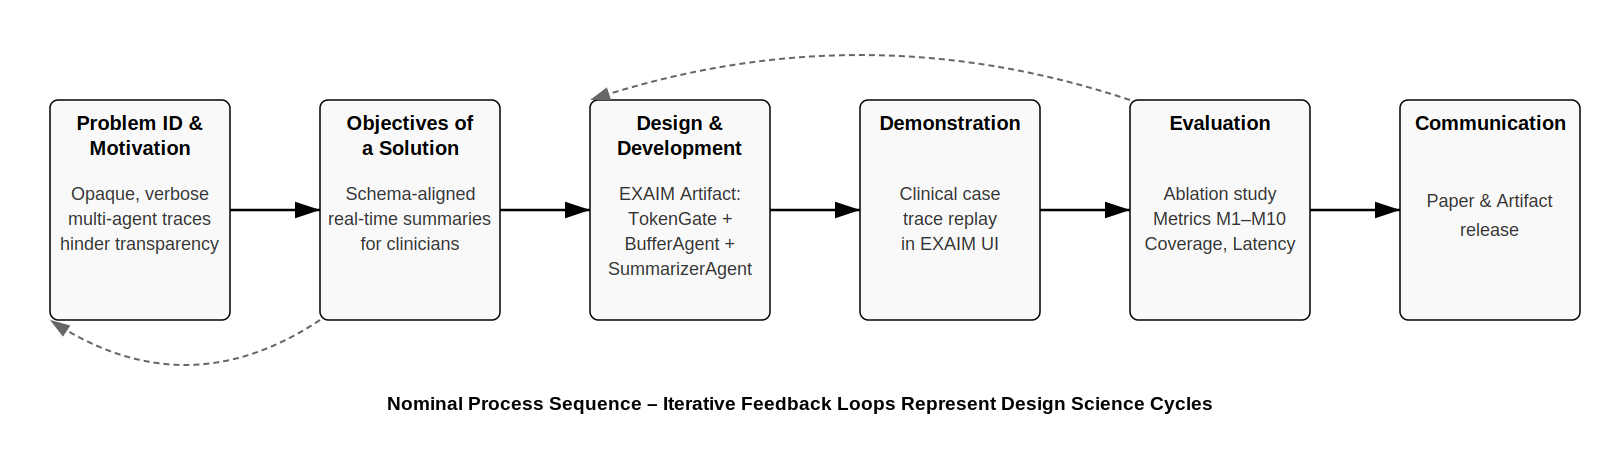
\includegraphics[width=\textwidth]{dsr/DSR.pdf}
\caption{EXAIM Design Science Research Methodology (DSRM) process model showing the six stages of our research lifecycle and the process iteration feedback loops.}
\label{fig:dsr}
\end{figure*}

We mapped the six DSRM steps to our research as follows: (1) Problem Identification: The introduction highlights the lack of real-time transparency in multi-agent CDSS (2) Objectives: Our research questions are centered around proposing and validating a structured artifact that produces more effective and contextual summarizations. (3) Design \& Development: The research objectives informed the design of the EXAIM artifact. (4) Demonstration: The EXAIM artifact was instantiated and successfully completed a clinical case walkthrough. (5) Evaluation: Following the demonstration, the artifact was evaluated using a controlled ablation study. (6) Communication: This paper serves as the dissemination artifact for the scientific community.

\section{Artifact Design}

\subsection{Design Objectives \& Rationale}

The design of EXAIM prioritizes timely, clinically meaningful communication under strict brevity and update-frequency constraints. This subsection articulates the key design decisions underlying the architecture and their theoretical and practical justification.

\subsection{System Architecture}

A foundational design decision for EXAIM is to implement as middleware rather than within individual diagnostic agents. Embedding explainability mechanisms directly into prompts or reasoning risks obfuscating transparency with diagnostic performance \cite{chen2025enhancing}. This limitation complicates validation and limits portability. By positioning EXAIM as an intermediary layer, explainability is decoupled from reasoning generation. This separation enables independent evolution of diagnostic agents and explanation mechanisms, supports integration with heterogeneous multi-agent frameworks, and preserves upstream system behavior. Middleware-level intervention also allows EXAIM to observe the full interaction among agents, rather than isolated reasoning fragments, which is essential for process-level transparency.

\subsection{Semantic-Driven Update Strategy}

EXAIM's update mechanism operates on semantic content rather than structural or mechanical properties, addressing both when to trigger updates and how to evaluate content relevance. Traditional approaches rely on either turn boundaries or fixed thresholds—both of which are poor proxies for semantic progression in multi-agent LLM systems. Turn-based summarization assumes that agent turn boundaries correspond to meaningful semantic transitions, but a single agent turn may contain exploratory reasoning, multiple topic transitions, or internal debate, whereas clinically meaningful changes may occur mid-turn. Similarly, fixed thresholds—such as token counts or time intervals—are computationally simple but insensitive to content, often producing fragmented or repetitive updates.

EXAIM therefore adopts a unified semantic-driven strategy that addresses both timing and content evaluation. For update timing, EXAIM uses an event-driven approach in which summaries are triggered by semantic change rather than generation mechanics. This design aligns updates with clinically salient moments, such as the emergence of new evidence, shifts in diagnostic focus, or safety-critical findings. For content evaluation, EXAIM assesses semantic properties of the reasoning stream—including completeness, relevance, and novelty—rather than relying on heuristic thresholds. This filtering strategy allows the middleware to distinguish between verbosity and progression, suppressing repetitive grounding statements while surfacing genuinely new diagnostic information. By decoupling update timing from turn structure and content evaluation from mechanical thresholds, EXAIM aims to avoid lossy compression and reduce redundant updates compared to turn-based approaches, while also enabling adaptation to variability in agent behavior, case complexity, and reasoning style without requiring manual retuning of thresholds for each deployment. Together, these design decisions position semantic content as the primary signal for update decisions, ensuring that transparency mechanisms respond to meaningful clinical progression rather than structural artifacts of the reasoning process.

\subsection{Novelty Gating for Update Stream Control}

A key design insight in EXAIM is that redundancy reduction alone is insufficient for managing update frequency and marginal-information emissions. Multi-agent systems may produce a sequence of distinct yet marginally informative updates that are technically non-redundant but represent low marginal-information emissions. To address this, EXAIM explicitly incorporates novelty as a gating criterion. Novelty is evaluated relative to previously surfaced summaries rather than raw agent output, allowing the system to suppress low-impact incremental updates until sufficient informational value has accumulated. This design trades marginal gains in information coverage for substantial reductions in interruption frequency, aligning with evidence-based principles for alert fatigue mitigation in clinical systems.

\subsection{Schema-Constrained Summarization and Bounded Output Budgets}

To bridge the gap between verbose agent reasoning and real-time clinical needs, EXAIM enforces a structured summary schema. The design addresses two competing requirements: (1) Structural Predictability, achieved by mapping fields to established clinical mental models (SBAR and SOAP) \cite{haig2006sbar,podder2023soap,marcilly2018alerts}, and (2) Bounded Information Density, achieved by enforcing strict ``output budgets'' for each field.

Rather than relying on open-ended generation, we define fixed character budgets that function as a bounded UI contract. These limits act as engineering constraints to operationalize qualitative usability principles—such as ``brief titles'' \cite{pourian2025alerts} or ``short snippets'' \cite{vanveen2023summarization}—into a deterministic system property. This ensures that the middleware produces a stable, scannable interface footprint that does not fluctuate with model verbosity. Table~\ref{tab:schema} details the schema and the design heuristics motivating each budget.

\begin{table*}[htbp]
\caption{EXAIM Summary Schema: Clinical Mapping and Bounded Output Budgets}
\label{tab:schema}
\begin{center}
\renewcommand{\arraystretch}{1.3}
\begin{tabular}{p{2.5cm}p{2.5cm}p{4cm}p{1.5cm}p{4.5cm}}
\toprule
\textbf{Field} & \textbf{Clinical Map} & \textbf{Role} & \textbf{Budget (Chars)} & \textbf{Design Motivation} \\
\midrule
Status / Action & SBAR: Situation & Alert header; scannable update. & 150 chars & Enforces scannability via brief title heuristic \cite{pourian2025alerts}. \\
Key Findings & SOAP: Obj/Subj & Salient facts; ``live snippet'' paradigm. & 180 chars & Supports $\sim$2 concise snippets aligned with targeted summarization limits \cite{vanveen2023summarization}. Structured presentation addresses transparency barriers identified in patient-centered CDSS deployment \cite{harrison2022patient}. \\
Differential & SOAP: Assessment & Diagnostic interpretation. & 210 chars & Bounds complexity to maintain interpretability \cite{lage2019interpretability}. \\
Uncertainty & SOAP: Assessment & Explicit confidence signal. & 120 chars & Simplified framing for trust calibration \cite{goel2022covid}. \\
Rec. / Plan & SOAP: Plan & Actionable next step. & 180 chars & Action-linked explanations \cite{silva2023xai,bergomi2022impact}. \\
Agent Contrib. & System Meta & Attribution of active agents. & 150 chars & Pipeline transparency patterns \cite{donadello2021sexai}. \\
\bottomrule
\end{tabular}
\end{center}
\footnotesize
Note: Character budgets are hard constraints that enforce a bounded UI contract, ensuring stable interface footprint regardless of model verbosity.
\normalsize
\end{table*}

\subsection{EXAIM Architecture}

EXAIM follows an event-driven architecture composed of three sequential components: (1) a TokenGate for syntax-aware stream regulation, (2) a BufferAgent for semantic event detection, and (3) a SummarizerAgent for schema-constrained synthesis. Each component progressively increases the semantic abstraction of the incoming data while enforcing strictly defined flow-control policies.

\subsubsection{Middleware Placement and Data Flow}

EXAIM is positioned downstream of all diagnostic agents and upstream of the clinician-facing interface. The system operates on a ``push'' model where agents emit tokens asynchronously to the middleware. Unlike turn-based systems that rely on orchestration artifacts (e.g., turn\_end events), EXAIM intercepts the raw token stream, allowing it to operate at a finer granularity than conventional conversational interfaces. The middleware maintains no global diagnostic authority; instead, it functions as an interpretive layer that monitors reasoning progression and emits summaries only when specific semantic thresholds are crossed.

\subsubsection{Syntax-Aware Stream Regulation (TokenGate)}

The first stage of the EXAIM pipeline regulates the high-velocity output of large language models into semantically coherent segments suitable for downstream analysis. Raw token streams produced by LLMs are often fragmented, bursty, and misaligned with linguistic boundaries. Processing such streams directly leads to excessive summarization triggers or incomplete semantic units.

To maintain low latency and avoid dependencies on model-specific tokenizers (e.g., BPE, TikToken), TokenGate operates on whitespace-delimited word counts. The TokenGate accumulates tokens into a per-agent buffer and flushes only when specific structural or temporal conditions are met. These flush policies are prioritized to balance latency with linguistic integrity:

\begin{itemize}
\item \textbf{Boundary-Aware Accumulation:} To prevent severing sentences mid-thought, the gate accumulates tokens until a minimum word threshold (min\_words=60) is met and a boundary cue is detected. We employ a regex pattern that targets sentence-terminating punctuation followed by optional closures: \verb|r"[.?!][)\]\}\'\"]*$"|.
\item \textbf{Silence Detection:} To handle bursty agent behavior, a silence\_timer (1.0s) forces a flush if no new tokens are received, preventing data from becoming ``stuck'' during agent retrieval pauses.
\item \textbf{Safety Valves:} To guarantee upper-bound latency during verbose generation, a hard flush is forced if the buffer exceeds max\_words=100 or a max\_wait\_timeout of 4.0s, regardless of boundary cues.
\end{itemize}

These parameter values were selected through systematic calibration across 625 policy combinations using multi-objective optimization (see Section V.A.1).

\subsubsection{Semantic Buffering and Event Detection (BufferAgent)}

The core innovation of EXAIM lies in its semantic buffering layer, which determines when a clinician-facing update should be generated. Rather than triggering summaries at fixed intervals or agent turn boundaries, EXAIM evaluates the semantic content of buffered segments to detect meaningful reasoning events.

This component analyzes incoming segments using a structured BufferAnalysis state machine, classifying the stream into one of three states:
\begin{itemize}
\item \textbf{SAME\_TOPIC\_CONTINUING:} Elaboration on a previous concept
\item \textbf{TOPIC\_SHIFT:} Movement to a new clinical domain or reasoning phase
\item \textbf{CRITICAL\_ALERT:} High-priority clinical event requiring immediate attention
\end{itemize}

Beyond state classification, the BufferAgent assesses incoming segments along three dimensions:
\begin{itemize}
\item \textbf{Completeness:} whether the segment represents a finished clinical thought rather than an incomplete clause or speculative fragment.
\item \textbf{Relevance:} whether the content contributes to clinically meaningful information, as opposed to internal agent coordination or procedural reasoning.
\item \textbf{Novelty:} whether the information introduces new diagnostic insight relative to previously surfaced summaries.
\end{itemize}

Based on this semantic assessment, the middleware decides whether to trigger summarization or continue accumulating context. Crucially, EXAIM distinguishes verbosity from progression. Multi-agent systems often restate known facts to ground internal reasoning; such repetition is filtered to avoid redundant clinician notifications. At the same time, EXAIM ensures that clinically significant transitions—such as changes in diagnostic focus or emergent safety concerns—are surfaced promptly.

\subsubsection{Schema-Constrained Clinical Summarization (SummarizerAgent)}

When a semantic event is detected, the accumulated context is passed to the summarization layer. This component generates a concise, structured update that reflects the current state of multi-agent reasoning rather than a retrospective summary of the entire case. Summaries are constrained to a fixed schema aligned with established clinical communication frameworks (e.g., SBAR/SOAP). Each summary captures: (i) the current diagnostic status or action, (ii) key clinical findings, (iii) rationale for leading hypotheses, (iv) uncertainty or confidence considerations, (v) recommended next steps, and (vi) attribution of contributing agents.

Strict structural and length constraints are enforced to ensure consistency, readability, and predictable output contracts. The summarization layer is explicitly prohibited from inventing or extrapolating information beyond the provided context. If no new information is available for a given field, the summary reflects this absence rather than repeating prior content. By enforcing schema-level constraints, EXAIM produces updates that are predictable in form, comparable over time, and suitable for integration into clinician-facing dashboards or electronic health record workflows.

\begin{figure*}[htbp]
    \centering
    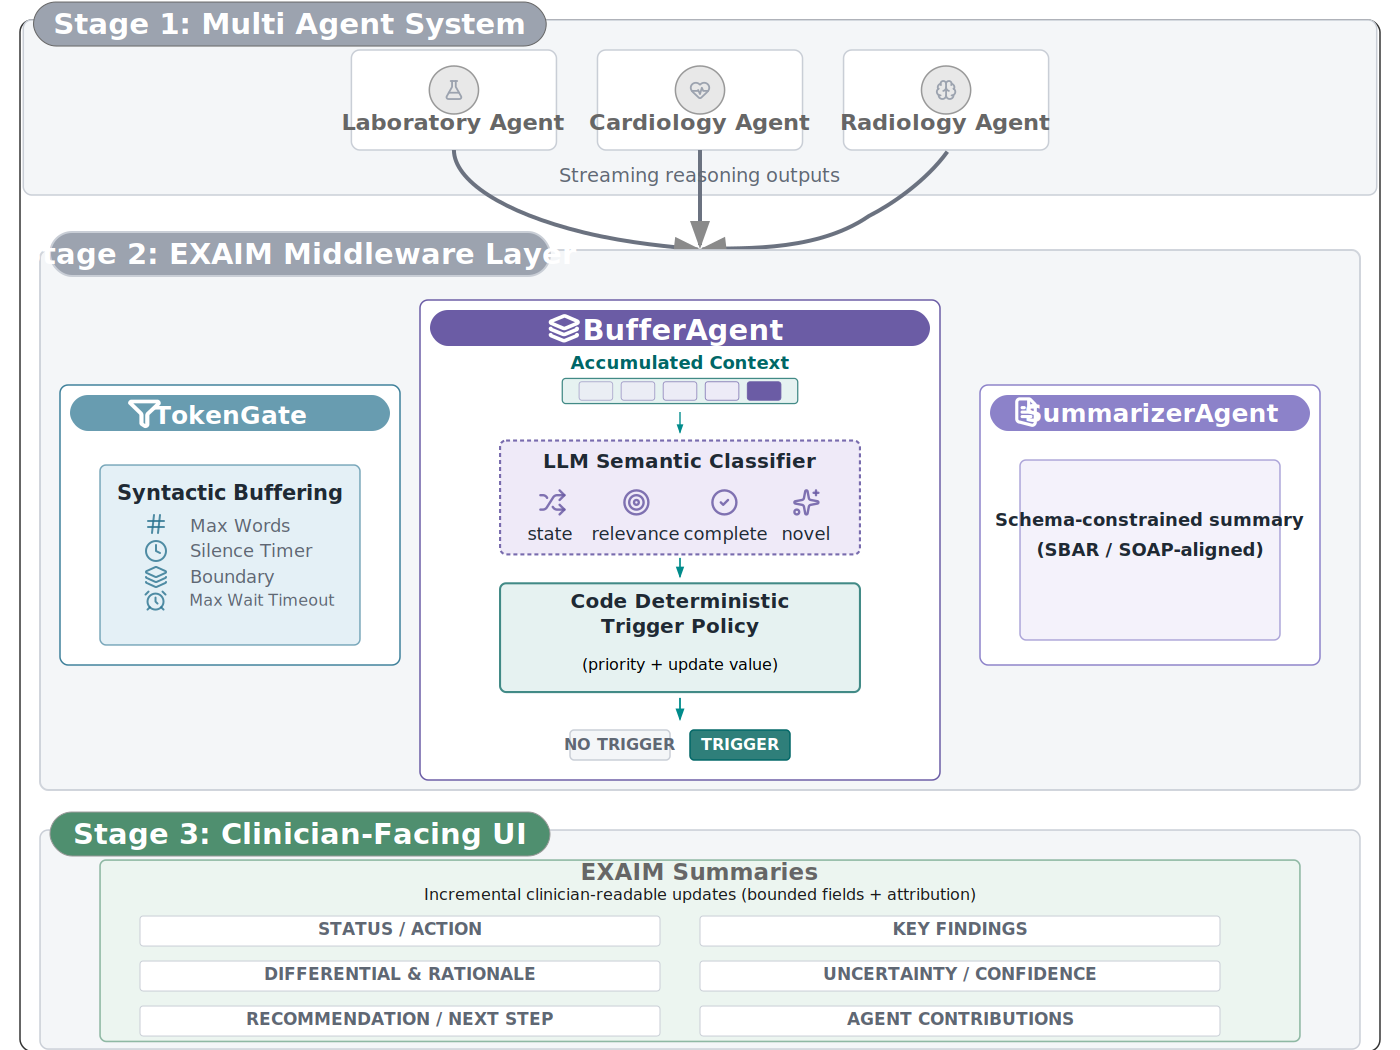
\includegraphics[width=\textwidth]{../raw/systemFigure/system.pdf}
    \caption{EXAIM System Architecture Overview showing the three-stage pipeline: (1) Stage 1: Interleaved Input Stream from external agents (Laboratory, Cardiology, Radiology), (2) Stage 2: EXAIM Middleware Layer with TokenGate (syntax-aware buffering), BufferAgent (semantic boundary detection), and SummarizerAgent (schema-constrained compression), and (3) Stage 3: Structured Output in SBAR/SOAP format. The diagram illustrates the flow of streaming token deltas through the middleware, semantic event detection, and the generation of coherent, bounded summaries for clinician-facing interfaces.}
    \label{fig:system-architecture}
\end{figure*}

\subsubsection{Case Walkthrough}

To demonstrate EXAIM's semantic filtering and redundancy detection mechanisms, we analyze a specific interaction sequence from a multi-agent reasoning trace (Case ID: 3949). This trace was generated using the MAC Framework (described in Section V-A), which simulates a team of diagnostic agents collaborating on a complex medical case.

\textbf{1. Context State (Pre-Condition)} Prior to this segment, doctor0 and doctor1 had already established Spinocerebellar Ataxia (SCA) as the leading diagnosis. The middleware had generated summaries capturing this consensus and the recommended genetic tests (Log ID: summary\_3). The active buffer was empty.

\textbf{2. The Raw Input Stream} doctor2 then enters the discussion. The agent generates a verbose response concurring with the previous agents and re-stating the established diagnosis.

\textit{Raw Trace (doctor2):} ``\textit{\#\#\# Most Likely Diagnosis: Spinocerebellar Ataxia (SCA): I concur with both Doctor0 and Doctor1 that the most likely diagnosis is spinocerebellar ataxia... The gradual onset at age 30 years also aligns with hereditary SCAs... \#\#\# Differential Diagnoses: 1. Multiple Systems Atrophy (MSA): While I agree that MSA typically presents with...}''

\textbf{3. BufferAgent Logic (Internal Rationale)} While the dashboard remained visually static (see Fig.~\ref{fig:suppression-demo}), the middleware was actively analyzing the stream. As visualized in Fig.~\ref{fig:logic-card}, the system detected semantic redundancy through its multi-stage evaluation process. Despite the input's clinical relevance, the novelty check failed, causing the middleware to suppress the update and prevent redundancy.

\begin{figure}[h]
    \centering
    \begin{tcolorbox}[
        enhanced,
        colback=white,
        colframe=black,
        boxrule=0.5mm,
        arc=2mm,
        drop shadow,
        left=4mm,
        right=4mm,
        top=2mm,
        bottom=2mm,
        title=\textbf{BufferAgent Status [doctor2]},
        fonttitle=\bfseries\normalsize,
        coltitle=black,
        colbacktitle=white,
        halign title=center,
        fontupper=\normalsize
    ]
        \normalsize
        
        \textbf{Input Stream:}
        \vspace{-1mm}
        \begin{quote}
            \itshape "...I concur with both Doctor0 and Doctor1... adding no new information."
        \end{quote}
        \vspace{1.5mm}
        
        \textbf{Decision Flags:}
        \vspace{0.5mm}
        
        \begin{center}
        \begin{tabular}{@{}c@{}}
            \raisebox{5pt}{State} \\
            \tcbox[colback=churkinpurple!15, colframe=churkinpurple, size=small, boxrule=0.5mm, left=2mm, right=2mm, top=0.5mm, bottom=0.5mm, fontupper=\normalsize]{\textcolor{churkinpurple}{\texttt{SAME\_TOPIC\_CONTINUING}}}
        \end{tabular}
        \end{center}
        
        \vspace{0.1mm}
        \begin{center}
        \begin{tabular}{@{}c@{\hspace{2mm}}c@{\hspace{2mm}}c@{}}
            \begin{tabular}{@{}c@{}}
                \raisebox{5pt}{Complete} \\[-3pt]
                \tcbox[colback=statusgreen!15, colframe=statusgreen, size=small, boxrule=0.5mm, left=2mm, right=2mm, top=0.2mm, bottom=0.2mm, fontupper=\normalsize]{\textcolor{statusgreen}{\textbf{True}}}
            \end{tabular} &
            \begin{tabular}{@{}c@{}}
                \raisebox{5pt}{Relevant} \\[-3pt]
                \tcbox[colback=statusgreen!15, colframe=statusgreen, size=small, boxrule=0.5mm, left=2mm, right=2mm, top=0.2mm, bottom=0.2mm, fontupper=\normalsize]{\textcolor{statusgreen}{\textbf{True}}}
            \end{tabular} &
            \begin{tabular}{@{}c@{}}
                \raisebox{5pt}{Novel} \\[-3pt]
                \tcbox[colback=statusred!15, colframe=statusred, size=small, boxrule=0.5mm, left=2mm, right=2mm, top=0.2mm, bottom=0.2mm, fontupper=\normalsize]{\textcolor{statusred}{\textbf{False}}}
            \end{tabular} \\
        \end{tabular}
        \end{center}
        \vspace{-2mm}
        \begin{center}
            $\downarrow$
        \end{center}
        \vspace{-2mm}
        \begin{center}
            \tcbox[
                enhanced,
                colback=statusred!20,
                colframe=statusred,
                boxrule=0.5mm,
                size=normal,
                fontupper=\bfseries\normalsize,
                left=3mm,
                right=3mm,
                top=0.5mm,
                bottom=0.5mm
            ]{\textcolor{statusred}{Trigger = False (Suppressed)}}
        \end{center}
        
        \vspace{0.1mm}
        \noindent\rule{\linewidth}{0.5mm}
        \vspace{0.5mm}
        
        \textbf{Rationale:} Doctor2 concurs with SCA based on ataxia/dysarthria/MRI... adding no new information. The content is \textcolor{statusgreen}{relevant} as it details planned actions, but it is \textcolor{statusred}{not novel} as these details were already broadly mentioned in previous summaries.
    \end{tcolorbox}
    \caption{BufferAgent System Status Card showing the hierarchical decision logic. Three evaluation conditions (\textcolor{statusgreen}{Complete=True}, \textcolor{statusgreen}{Relevant=True}, \textcolor{statusred}{Novel=False}) combine to produce the final result: \textcolor{statusred}{Trigger=False (Suppressed)}, preventing redundant update generation.}
    \label{fig:logic-card}
\end{figure}

\begin{figure*}[htbp]
\centering
\includegraphics[width=\textwidth]{case_walkthrough/CaseWalkthroughImage.png}
\caption{The EXAIM dashboard during redundancy suppression. The left panel shows the raw, verbose stream from doctor2 concurring with the diagnosis. The right panel remains static (displaying the previous doctor1 update), visually confirming that the middleware successfully filtered the non-novel content.}
\label{fig:suppression-demo}
\end{figure*}

\textbf{4. Outcome} Consequently, EXAIM filtered this update, preventing the generation of a low-value summary. The middleware continued to buffer doctor2's subsequent tokens silently until the agent introduced specific new details regarding ``High-Resolution MRI techniques'' and ``Oligoclonal bands,'' which finally triggered a consolidated, high-density update.

\section{Evaluation}

To isolate the architectural contribution of EXAIM, we employ a ``glass-box'' evaluation methodology using deterministic replays of multi-agent reasoning traces. This approach allows us to stress-test the middleware's flow-control capabilities independent of variations in upstream agent behavior. The evaluation employs automated metrics to enable reproducible, systematic comparison across variants, aligning with established frameworks for XAI evaluation that emphasize both technical performance and user-centered criteria \cite{vilone2021explainable}.

\subsection{Experimental Setting}

To evaluate the EXAIM middleware, we utilized the Multi-Agent Conversation (MAC) framework (Chen et al., 2025) as the upstream trace generator. MAC is a multi-agent diagnostic system where diverse doctor agents and a supervisor collaborate to solve medical cases.

For this study, we instrumented the MAC framework to capture the real-time dynamics of these multi-agent interactions. Specifically, we modified the upstream codebase to log granular stream deltas (chunk-level text outputs) and precise generation timestamps (both absolute and relative to the turn start) during the agent reasoning process. This instrumentation enables us to capture the exact cadence of token generation without altering the agents' underlying prompts, roles, or decision-making logic.

The resulting outputs are stored as frozen replay traces. These traces allow us to simulate a live stream deterministically, feeding identical token sequences and timing delays into the EXAIM middleware across all experimental runs. This decoupling ensures that any measured variance in latency or summarization quality is attributable solely to the EXAIM configuration, rather than stochastic variations in the upstream diagnostic agents.

\subsubsection{TokenGate Parameter Calibration}

The TokenGate component requires four configurable parameters: minimum word threshold (min\_words), maximum word threshold (max\_words), silence detection timer (silence\_timer), and maximum wait timeout (max\_wait\_timeout). To ensure reproducible parameter selection, we conducted systematic calibration across a grid of 625 policy combinations evaluated on frozen replay traces. Table~\ref{tab:tokengate-grid} shows the parameter ranges explored in the calibration grid, with validity constraints ensuring min\_words $<$ max\_words and max\_wait\_timeout $\geq$ silence\_timer.

\begin{table}[htbp]
\caption{TokenGate Parameter Calibration Grid}
\begin{center}
\renewcommand{\arraystretch}{1.3}
\begin{tabular}{lc}
\toprule
\textbf{Parameter} & \textbf{Values Tested} \\
\midrule
min\_words & 30, 40, 50, 60, 70 \\
max\_words & 80, 100, 120, 140, 160 \\
silence\_timer (seconds) & 1.0, 1.5, 2.0, 2.5, 3.0 \\
max\_wait\_timeout (seconds) & 4.0, 5.0, 6.0, 7.0, 8.0 \\
\bottomrule
\end{tabular}
\label{tab:tokengate-grid}
\end{center}
\end{table}

Each policy was evaluated using metrics that balance latency, computational cost, and semantic coherence: time-to-first-flush (TTFF), average flush frequency per case, median chunk size, spam percentage (flushes below 70\% of min\_words threshold), and worst-case wait times. Policies were filtered through hard constraints: spam percentage $\leq$ 10\%, timer-triggered flushes below min\_words $\leq$ 20\%, median chunk size $\geq$ 50 words, flush count $\leq$ 100 per case, and maximum chunk size $\leq$ 180 words. Derived constraints from trace timing distributions were also applied to ensure policies respect realistic token generation cadences.

From the surviving policies that passed all constraints, selection employed a three-objective Pareto frontier analysis optimizing simultaneously for low TTFF, low flush frequency, and high median chunk size. Objectives were normalized to a [0,1] goodness space using percentile-based bounds computed from survivor policies. The policy with minimum dimension-normalized Euclidean distance to the utopia point (1, 1, 1) was selected, ensuring balanced optimization across all three objectives. This process selected min\_words=60, max\_words=100, silence\_timer=1.0s, and max\_wait\_timeout=4.0s, which balance low latency (rapid first flush), moderate flush frequency (reducing BufferAgent computational overhead), and semantic coherence (sufficient chunk size for meaningful boundary detection).

\subsubsection{EXAIM Implementation Details}

To ensure reproducibility and isolate the middleware's contribution from stochastic model variance, we enforce strict configuration constraints:

\begin{itemize}
\item \textbf{Middleware Model and Deterministic Sampling:} Both the BufferAgent (trigger logic) and SummarizerAgent (synthesis) are powered by Gemini 2.5 Flash Lite (Google), selected for its high throughput and native support for large context windows. All middleware components operate at temperature=0.0 to minimize generation variance and ensure deterministic, reproducible outputs.
\item \textbf{Constraint Enforcement:} Schema validation and character-limit truncation are enforced using Pydantic v2 models with LangChain's structured output (strict=True). The SummarizerAgent employs a three-attempt strategy: initial structured output, retry with rewrite prompt for length violations, and fallback truncation. If validation fails after all attempts, an empty summary is generated and marked as failed (schema\_ok=false) for metrics exclusion, ensuring the system continues operation while tracking failure rates.
    \item \textbf{Metric Extraction:} For semantic evaluation, we utilize scispaCy (en\_core\_sci\_sm) with the UMLS Entity Linker to extract canonical medical concepts (CUIs) from both the raw traces and generated summaries.
    \item \textbf{LLM Usage Measurement (M9):} Token-equivalent estimates (CTU) report user prompt and completion text only, excluding fixed system prompts. System prompts are constant across variants and represent fixed infrastructure overhead rather than variable computational cost per decision.
\end{itemize}

\subsubsection{Ablation Variants}

To isolate the contribution of individual architectural components, we conduct a controlled ablation study comparing the full EXAIM system (V0) against four structural variants: (1) V1 (Turn-End Baseline): Summarization triggered only at agent turn boundaries, without TokenGate or BufferAgent; (2) V2 (No BufferAgent): TokenGate segmentation without semantic buffering, resulting in frequent updates; (3) V3 (Fixed-Chunk): BufferAgent with novelty filtering but fixed-size chunking instead of syntax-aware segmentation; and (4) V4 (No Novelty): Full EXAIM architecture without novelty gating. All variants use the same summarization schema to ensure comparability.

\subsubsection{Evaluation Metrics}

We assessed EXAIM using a hierarchy of ten metrics (M1--M10), distinguishing between primary performance indicators and supplementary contextual measures. All token volume metrics (M2, M7, M9) report CTU (Character-Normalized Token Units), computed as $\lceil \text{len(text)} / 4 \rceil$. This vendor-agnostic, deterministic unit provides a token-equivalent estimate that enables consistent measurement across different LLM providers and tokenization schemes.

\paragraph{Primary Metrics}

We prioritized five metrics that directly quantify utility and reliability proxies:

\begin{itemize}
    \item \textbf{Strict Faithfulness (M6b):} The semantic alignment between the summary and the ground-truth reasoning trace. Higher scores indicate stronger contract-grounded alignment under a strict concept-realization proxy and are intended to penalize unsupported insertions. Faithfulness is a standard evaluation criterion in human-in-the-loop dialogue systems \cite{chen2022hitl}.
    \item \textbf{Redundancy Reduction (M3):} Measured via Jaccard similarity between consecutive summary updates:
    \begin{equation}
    J(S_i, S_{i+1}) = \frac{|C_i \cap C_{i+1}|}{|C_i \cup C_{i+1}|}
    \end{equation}
    where $C_i$ and $C_{i+1}$ are the sets of unique UMLS concepts (CUIs) extracted from summaries $S_i$ and $S_{i+1}$. Lower scores indicate the successful suppression of repetitive content (solving the verbosity problem).
    \item \textbf{Trace Coverage (M4):} The fraction of unique CUIs from the union of all summaries that are present in the trace, computed as $|\text{summary\_CUIs} \cap \text{trace\_CUIs}| / |\text{trace\_CUIs}|$, where trace\_CUIs is the set of unique CUIs extracted from the entire case trace, ensuring that conciseness does not result in critical information loss.
    \item \textbf{System Latency (M8):} The end-to-end processing time (buffer analysis + summarization generation) to validate the ``real-time'' architectural claim. We report mean, p50 (median), and p95 percentiles across all summary events, as tail latencies are critical for streaming system performance.
    \item \textbf{Schema Compliance (M10):} The rate of successful adherence to the JSON clinical output schema, verifying the system's structural reliability.
\end{itemize}

\paragraph{Supplementary Metrics}

To provide a holistic view of system behavior, we report five additional metrics in Table~\ref{tab:supplementary-metrics}. These include \textbf{Update Frequency (M1)} and \textbf{Token Volume (M2)}, which provide context for the coverage scores; \textbf{Unsupported Concept Fraction (M5)}, the fraction of concepts extracted from summaries that are not found in the trace under strict UMLS linking; \textbf{Contextual Faithfulness (M6a)}; and \textbf{Budget Efficiency (M7)}, which offers granular insights into token economics. M5 is highly sensitive to extraction/linking failures and surface-form changes (abbreviation, normalization, compression) rather than measuring actual hallucination. Its near-constant values across variants (~0.60) reflect systematic extraction artifacts rather than variant-specific differences.

\subsubsection{Limitations of Concept-Level Faithfulness Metrics in Compressed Clinical Summaries}

Our faithfulness metrics (M6a, M6b) operate at the level of explicit concept realization rather than semantic equivalence or entailment. This design choice introduces a fundamental structural mismatch between what summarization accomplishes and what strict concept-overlap metrics measure.

Schema-constrained summarization necessarily introduces several transformations that systematically reduce recall under strict NER-based concept matching: (1) \textbf{Abbreviation}, where full clinical phrases (e.g., ``acute renal failure'') are compressed to canonical forms (e.g., ``AKI''); (2) \textbf{Normalization}, where hedged or qualified statements (e.g., ``no evidence of infection'') are restated as direct assertions (e.g., ``infection unlikely''); (3) \textbf{Compression}, where modifiers, qualifiers, and redundant descriptors are omitted to meet character limits; and (4) \textbf{Schema remapping}, where clinical facts are reorganized into SBAR/SOAP slots, potentially altering surface forms.

In contrast, UMLS-based NER and concept linking typically assume explicit lexical realization, canonical surface forms, and near-literal mention of clinical entities. These assumptions align poorly with compressed summaries, where semantic content is preserved through paraphrase and structural reorganization rather than verbatim concept repetition. Consequently, a schema-constrained summarizer is guaranteed to under-score on strict concept-overlap metrics, even when the summary accurately represents the clinical content of the source trace.

Despite these limitations, concept-level faithfulness metrics remain informative for our evaluation. While absolute faithfulness scores are depressed by summarization effects, relative differences across ablation variants remain meaningful, as all systems are evaluated under identical extraction and linking assumptions. The metrics effectively capture hallucinated concepts not present in the trace, unsafe insertions (rather than omissions), and systematic differences in grounding quality across architectural variants. However, we do not claim that these metrics constitute a clinical safety guarantee or a substitute for human validation. Future work should incorporate clinician-judged factual consistency, sentence-level entailment verification, semantic similarity models, and task-based evaluation (e.g., decision agreement) to complement automated concept-level assessment.

\subsection{Results}

We target a streaming transparency regime that maximizes coverage and contract-grounded alignment under strict interruption (updates/case) and output budget constraints. While automated metrics provide reproducible, scalable evaluation of XAI systems, they should be complemented by human-centered evaluation for comprehensive assessment \cite{vilone2021explainable}. Table~\ref{tab:primary-metrics} presents the primary performance metrics comparing V0 (Full EXAIM) against all baseline variants. Table~\ref{tab:supplementary-metrics} provides supplementary contextual metrics for comprehensive analysis. Figure~\ref{fig:efficiency-frontier} visualizes the trade-off between interruption frequency and faithfulness, showing V0's position as a favorable operating point in the trade-off space.

\begin{table}[htbp]
\caption{Primary Performance Metrics: V0 vs. Baselines}
\begin{center}
\renewcommand{\arraystretch}{1.3}
\begin{tabular}{lccccc}
\toprule
\textbf{Metric} & \textbf{V0} & \textbf{V1} & \textbf{V2} & \textbf{V3} & \textbf{V4} \\
\midrule
Faithfulness (M6b) & 0.421 & 0.333 & 0.409 & 0.382 & 0.424 \\
Redundancy (M3) & 0.366 & 0.456 & 0.348 & 0.413 & 0.346 \\
Trace Coverage (M4) & 0.162 & 0.144 & 0.312 & 0.134 & 0.175 \\
Latency (M8, s) & & & & & \\
\quad Mean & 1.28 & 1.03 & 1.14 & 1.07 & 1.37 \\
\quad p50 & 1.22 & 0.96 & 1.06 & 1.04 & 1.33 \\
\quad p95 & 1.84 & 1.59 & 1.91 & 1.52 & 2.12 \\
Schema Compliance (M10) & 0.968 & 0.968 & 0.975 & 0.958 & 0.950 \\
\bottomrule
\end{tabular}
\label{tab:primary-metrics}
\end{center}
\end{table}

\begin{table}[htbp]
\caption{Supplementary Contextual Metrics}
\begin{center}
\resizebox{\columnwidth}{!}{%
\renewcommand{\arraystretch}{1.3}
\begin{tabular}{lccccc}
\toprule
\textbf{Metric} & \textbf{V0} & \textbf{V1} & \textbf{V2} & \textbf{V3} & \textbf{V4} \\
\midrule
Update Count (M1) & 11.7 & 8.5 & 46.4 & 9.5 & 16.5 \\
Output Volume (M2, CTU) & 1391 & 1148 & 4313 & 1156 & 1763 \\
Unsupported Fraction (M5) & 0.619 & 0.604 & 0.615 & 0.617 & 0.623 \\
Window-Groundedness (M6a) & 0.825 & 0.787 & 0.879 & 0.823 & 0.845 \\
Coverage @ 2000 CTU (M7) & 0.160 & 0.144 & 0.207 & 0.132 & 0.166 \\
LLM Usage (M9, CTU) & 62178 & 11618 & 37151 & 81694 & 58605 \\
\bottomrule
\end{tabular}%
}
\label{tab:supplementary-metrics}
\end{center}
\end{table}

\subsubsection{Full EXAIM vs. Turn-Based Baseline}

V0 improves strict faithfulness and reduces redundancy relative to V1, with modest coverage gains at a moderate latency cost. As discussed in Section V-A.5, absolute faithfulness scores are systematically depressed by summarization effects (abbreviation, normalization, compression, schema remapping); however, relative comparisons across variants remain informative under identical extraction assumptions.

\begin{figure}[htbp]
\centering
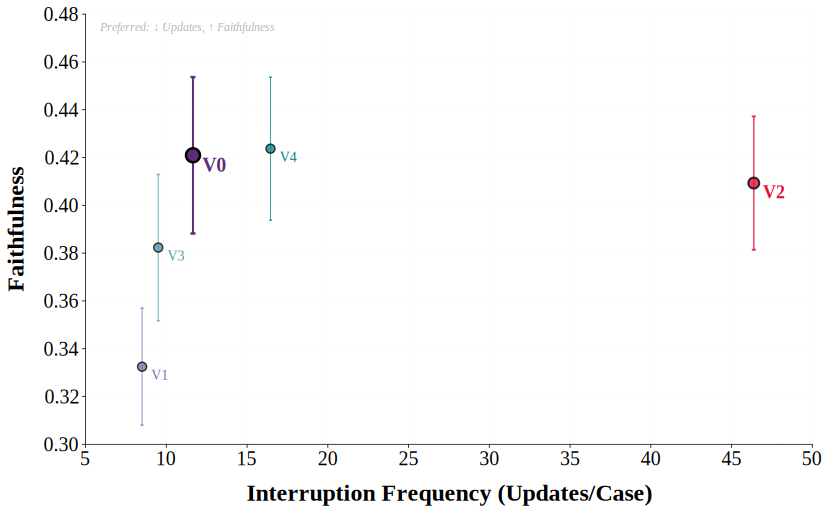
\includegraphics[width=\columnwidth]{efficiency_frontier/efficiency_frontier.pdf}
\caption{Trade-off between interruption frequency (updates per case) and faithfulness across ablation variants. Each point represents the mean over 40 cases; vertical bars indicate 95\% confidence intervals for faithfulness. V0 represents a balanced trade-off, achieving comparable faithfulness to higher-frequency baselines with substantially fewer updates. Lower update frequency and higher faithfulness are preferred.}
\label{fig:efficiency-frontier}
\end{figure}


While EXAIM generates more updates than V1, these updates contain higher informational value and less redundancy, representing a trade-off that balances update frequency with information density. Turn-based summarization compresses multi-topic agent turns into single summaries, leading to information loss and reduced grounding.

\subsubsection{Impact of Semantic Buffering}

Removing the semantic buffering layer (V2) results in a dramatic increase in update frequency (46.4 vs. 11.7 updates per case) and output volume (4313 vs. 1391 CTU). Without semantic filtering, the system produces excessive, fragmented updates, increasing update frequency and output volume and lowering semantic yield per update. This confirms that syntax-aware segmentation alone is insufficient for real-time explainability.

\subsubsection{Effect of Novelty Filtering}

Disabling novelty filtering (V4) increases update frequency (16.5 vs. 11.7 updates per case) without materially improving redundancy reduction (0.346 vs. 0.366). Although V4 captures marginally more information (coverage 0.175 vs. 0.162), it does so at the cost of higher interruption frequency. This demonstrates that novelty filtering functions as an update frequency control mechanism rather than a simple deduplication strategy.

\subsubsection{Adaptive vs. Fixed Segmentation}

Replacing syntax-aware segmentation with fixed-size chunking (V3) degrades both coverage (0.134 vs. 0.162) and faithfulness (0.382 vs. 0.421). Fixed segmentation frequently splits semantically complete reasoning units, forcing the summarizer to omit or infer missing context. Adaptive segmentation preserves logical coherence and improves grounding.

\subsubsection{Computational Overhead}

EXAIM introduces additional computational cost due to semantic analysis of the reasoning stream. Average summary latency increases from 1.03s (V1) to 1.28s (V0), with p95 tail latencies of 1.59s (V1) and 1.84s (V0). In streaming systems, tail latencies are critical for user experience; the observed p95 values remain within acceptable bounds for interactive dashboard update latencies. Total LLM token-equivalent usage (M9) increases by 5.3$\times$ (62,178 vs 11,618 CTU per case), reflecting the cost of semantic buffering and analysis. While LLM usage is higher, this overhead reflects the cost of semantic analysis required for redundancy suppression and improved contract-groundedness, at the cost of reduced coverage compared to higher-frequency variants.

\section{Discussion}

This work demonstrates that real-time explainability in multi-agent clinical decision support systems can be achieved through semantic-driven summarization that balances transparency with information density. EXAIM's design aligns with emerging principles for AI in clinical practice, which emphasize the need for systems that reduce cognitive load while maintaining transparency and supporting clinical workflow \cite{hor2025design}.
The results of this study highlight a fundamental mismatch between existing interaction abstractions and the operational realities of multi-agent clinical AI systems. In particular, they demonstrate that turn-based interfaces—while effective for human dialogue—are ill-suited for mediating transparency in distributed LLM reasoning environments. EXAIM's operating point advantage stems not from exposing more information, but from restructuring how and when information is surfaced.

\subsection{Rethinking Turns as a Transparency Primitive}

A central insight from the evaluation is that agent turns do not reliably correspond to semantic progression in multi-agent reasoning. Turn-based summarization compresses heterogeneous content into single updates, leading to reduced coverage and weaker grounding. Conversely, EXAIM's event-driven approach decouples explanation timing from generation mechanics, allowing clinically meaningful updates to be surfaced at sub-turn granularity. This finding suggests that explainability mechanisms should treat reasoning streams as continuous processes rather than discrete conversational exchanges. For system designers, this implies that transparency should be mediated by semantic state changes rather than orchestration artifacts.

\subsection{Semantic Buffering as Update Stream Control}

The ablation results demonstrate that semantic buffering is essential for balancing transparency and update frequency. Without semantic filtering, the system produces frequent, low-value updates that reduce information density; without novelty gating, it surfaces marginal informational gains at the cost of excessive interruption. EXAIM's buffering strategy effectively converts high-frequency, verbose reasoning streams into sparse, high-signal clinician-facing updates. This behavior positions EXAIM not as an explanation generator, but as an update stream control layer—one that regulates information flow through redundancy suppression and update frequency regularization. Such control is particularly important in high-stakes environments, where excessive transparency can be as operationally undesirable as insufficient transparency.

\subsection{Trade-offs Between Coverage and Update Frequency}

The evaluation reveals an inherent trade-off between maximal information coverage and interruption rate/output volume. Variants without novelty filtering achieve slightly higher coverage by surfacing incremental updates, but at the cost of higher interruption frequency. EXAIM explicitly prioritizes stream efficiency by suppressing low-impact updates, accepting a small reduction in total coverage to regularize update frequency. This trade-off reflects a broader principle in clinical system design: explainability must be selective rather than exhaustive. Transparency that increases update frequency and redundancy undermines its own operational value.

\subsection{Implications for Clinical AI System Design}

The findings suggest several implications for future clinical AI systems:
\begin{itemize}
\item Explainability should be treated as an independent architectural concern, separable from diagnostic reasoning.
\item Middleware layers provide a natural locus for managing transparency in complex, multi-agent systems.
\item Structured, schema-constrained explanations better support clinical sensemaking than free-form reasoning traces.
\item Incremental, event-driven disclosure aligns more closely with real-world clinical workflows than post-hoc summaries.
\end{itemize}

Collectively, these insights support a shift from explanation-as-output toward explanation-as-process in clinical AI design.

\section{Conclusion}

Multi-agent large language model systems offer powerful capabilities for clinical decision support, but their adoption is constrained by the difficulty of interpreting verbose, distributed reasoning processes in real time. Existing explainability approaches largely operate post hoc or expose raw reasoning traces without regard for update frequency and redundancy suppression, limiting their utility in time-sensitive clinical environments.

This paper introduced EXAIM, a real-time middleware architecture for process-level explainability in multi-agent clinical decision support systems. By decoupling transparency from diagnostic reasoning, EXAIM regulates streaming agent outputs through semantic event detection and schema-constrained summarization. The architecture enables incremental, clinician-aligned updates that preserve attribution and uncertainty while suppressing redundant or low-value information.

Through a controlled ablation study on multi-agent clinical reasoning traces, we demonstrated that semantic buffering achieves a better operating point for information coverage and faithfulness under interruption and budget constraints, with reduced redundancy compared to turn-based baselines. These gains are achieved with modest computational overhead, highlighting the feasibility of middleware-level explainability for real-world deployment.

More broadly, this work reframes explainability in clinical AI as a problem of information mediation rather than explanation exposure. As multi-agent systems become increasingly prevalent in high-stakes domains, architectures like EXAIM illustrate how real-time transparency can be achieved without inducing high-frequency, low-yield update streams or constraining upstream reasoning. Future clinical AI systems can build on this approach to deliver explainability that is not only faithful, but operationally effective.

\subsection{Limitations}

This study has several limitations that warrant consideration. First, the evaluation relies on replayed reasoning traces rather than live clinical deployment. While this approach enables controlled, reproducible comparison across variants, it does not capture downstream effects on clinician behavior, trust, or decision quality. As highlighted in patient-centered CDSS research, clinical effectiveness depends on integration with real-world workflows and clinician acceptance \cite{harrison2022patient}. Future work should incorporate human-in-the-loop evaluations to assess real-world impact.

Second, the dataset consists of rare-disease diagnostic cases, which tend to produce dense and exploratory reasoning traces. Performance characteristics may differ in routine clinical scenarios with more stable diagnostic trajectories. Further evaluation across diverse case types is needed to assess generalizability.

Third, semantic event detection in EXAIM relies on LLM-based analysis, which introduces additional computational cost. While the observed latency remains acceptable for reading tasks, future work could explore lightweight classifiers or distilled models to reduce overhead without sacrificing semantic sensitivity.

Finally, the evaluation employs automated proxy metrics to assess coverage, redundancy, and faithfulness. As detailed in Section V-A.5, concept-level faithfulness metrics operate at the level of explicit lexical realization rather than semantic equivalence, systematically under-scoring compressed summaries due to abbreviation, normalization, compression, and schema remapping. While relative comparisons across variants remain informative, these metrics cannot fully capture clinical nuance, contextual relevance, or semantic entailment. Complementary qualitative evaluation—including clinician-judged factual consistency, sentence-level entailment verification, and task-based assessment—will be necessary to validate the practical utility and safety of the system. Expert clinician evaluation has been successfully employed in prior work on LLM-based clinical summarization, providing validation of automated metrics through human judgment \cite{fraile2025llm}.

\section*{Acknowledgment}

The authors would like to thank the reviewers for their valuable feedback and suggestions.

\bibliographystyle{IEEEtran}
\bibliography{references}

\end{document}

